\begin{exr}
Se sap que una molècula gasosa de \ch{NaCl} té una distància interatòmica de 2.38\AA. Quina és l'energia potencial Coulòmbica d'un mol d'aquestes molècules?
\end{exr}
\begin{exr}
    Dedueix l'equació de Born-Mayer a partir de considerar, de forma simplificada, que l'energia d'atracció Coulòmbica es pot expressar com $-\frac{Me^2}{r}$ i que la repulsió entre ions es pot expressar com $\frac{B}{r^n}$.
    %U=-\frac{Me^2}{r_0}(1-1/n)
    \end{exr}
    \begin{exr}
    L'òxid de magnesi, \ch{MgO}, té la mateixa estructura que el \ch{NaCl}. Sabent que $r(\ch{Mg^{2+}})=72pm$ i que $r(\ch{O^{2-}})=140pm$, calcula l'energia de malla d'aquest compost iònic.
    %\includegraphics[scale=0.5]{res_ex1.png}
    %-3.84 10^3 kj mol-1
    \end{exr}
    
    \begin{exr}
    Fent servir el cicle de Born-Haber, estima l'entalpia de malla del \ch{KCl}.
    %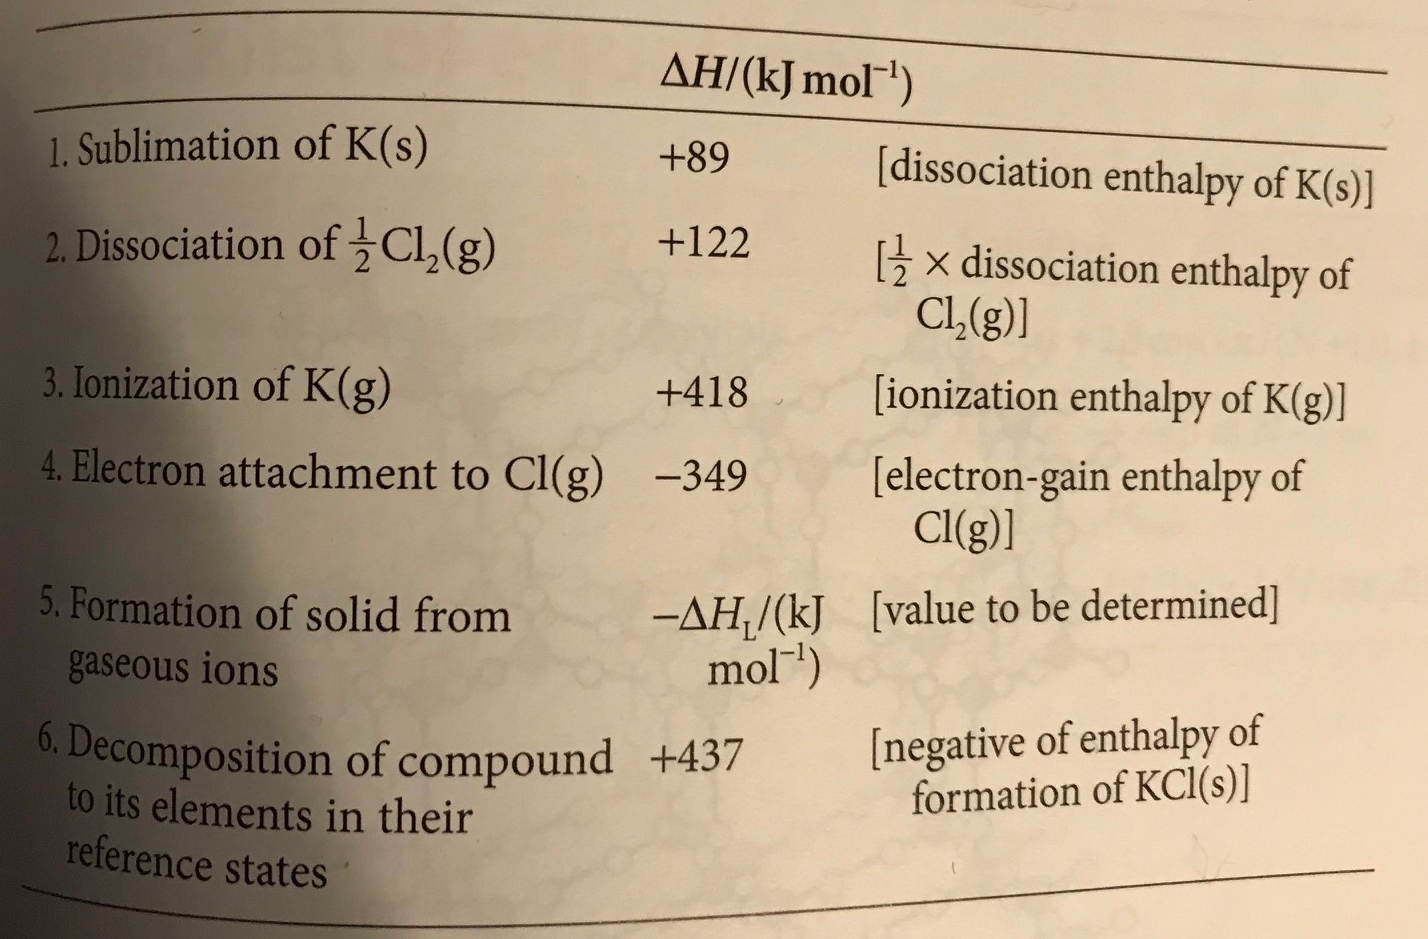
\includegraphics[scale=0.5]{res_ex2.png}
    %717 kj mol-1
    %exercici examen CaO (veure atkins)
    \end{exr}